\documentclass[10pt,conference,compsocconf]{IEEEtran}

\usepackage{hyperref}
\usepackage{graphicx}	% For figure environment
\usepackage{amsmath}
\usepackage{amssymb}
\usepackage{float}
\usepackage{url}
\newcommand{\beginsupplement}{%
	\setcounter{table}{0}
	\renewcommand{\thetable}{S\arabic{table}}%
	\setcounter{figure}{0}
	\renewcommand{\thefigure}{S\arabic{figure}}%
}

\begin{document}
\title{Extreme Wind Analysis}

\author{
	Matthias Minder, Yves Rychener
}

\maketitle

\begin{abstract}

\end{abstract}

\section*{Introduction} 
Modeling extreme weather events is of interest for a variety of applications, such as risk assessment for insurance companies or conception of preventive measures. In particular, questions about how often a particular event will occur, how severe events can get, and whether there are seasonal or year-dependent trends are of interest. Within the scope of this report, we will address these questions for extreme thunderstorms on a 1° longitude and 1° latitude grid cell with south-west coordinates 38° latitude and -100° longitude, situated in central Kansas. The measured quantities are the Connective Available Potential Energy ($CAPE$) and the Storm Relative Helicity ($SRH$), which have to be simultaneously high for severe thunderstorms to occur. Three-hourly time series of these events are taken into account from January 1st 1979 at 00:00 to December 31st 2015, 21:00. 
\par
In particular, we will study the value denoted $PROD$ given by $PROD = \sqrt{CAPE} \times SRH$. It captures concurrently high values of $SRH$ and $CAPE$, and is thus apt for modeling the risk of thunderstorms. Every month will be treated separately in order to capture seasonal differences. To model extreme values, a generalized extreme value distribution will be fitted to the monthly maxima of $PROD$ using maximum likelihood estimation as well as Bayesian approaches. Moreover, the generalized extreme value distribution will be fitted to the $r$-largest order statistic for every month to determine whether that improves the fit. Subsequently, we will assess dependence of $PROD$ upon time and the NINO 3.4 index, an established indicator of the El-Niño Southern Oscillation ($ENSO$). 
\par
Following this, $CAPE$ and $SRH$ are considered separately. We will study whether they are asymptotically dependent, before fitting bivariate models to the joint extremes of $CAPE$ and $SRH$. 
Finally, 50- and 100-year return levels of $PROD$ are calculated based on fitting a point process model to $PROD$ with maximum likelihood estimation, based on the Bayesian fit, and based on simulated values of $CAPE$ and $SRH$ from the bivariate model fitted before. 

\section*{Preliminary Analysis}
\begin{figure}
	\centering
	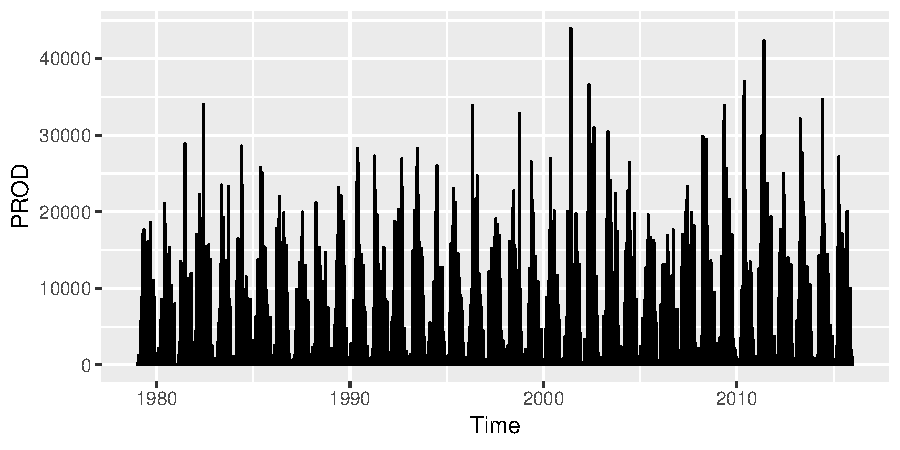
\includegraphics[width=0.35\textwidth]{../plots/full_time_series.pdf}
	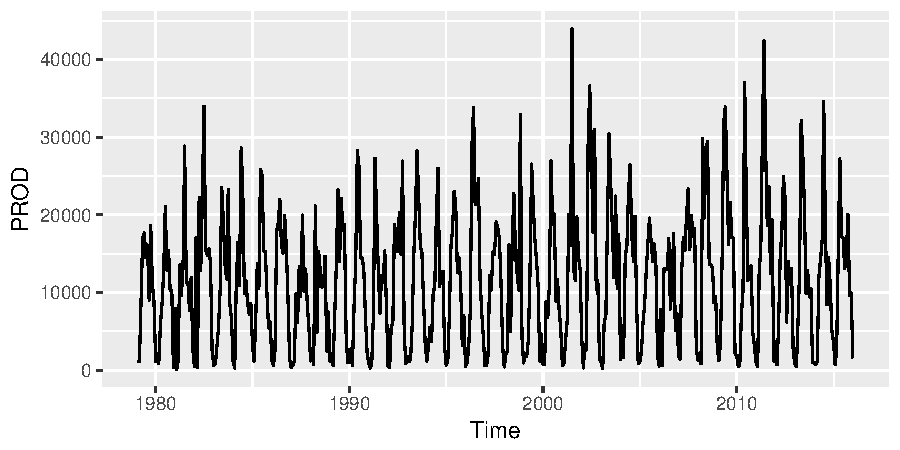
\includegraphics[width=0.35\textwidth]{../plots/monthly_max_series.pdf}
	\caption{Three-hourly values (top) and monthly maxima (bottom) of $PROD$ values for the entire analyzed period.}
	\label{fig:timeseries}
\end{figure}
Plotting the full time series and the monthly maxima as shown in Figure \ref{fig:timeseries} clearly shows the seasonality of the data, with high values of $PROD$ occurring mainly during summer. This clearly shows the necessity of separate treatment of months. Moreover, there seems to be some upward trend following time, with more extreme values of $PROD$ in recent years.

\section*{Fitting Generalized Extreme Value Distribution to PROD}
In order to understand the behavior of the monthly maxima, we fitted a generalized extreme value (GEV) distribution to $PROD$ for each month separately with three different approaches. 
\begin{figure}
	\centering
	\textbf{January}\\
	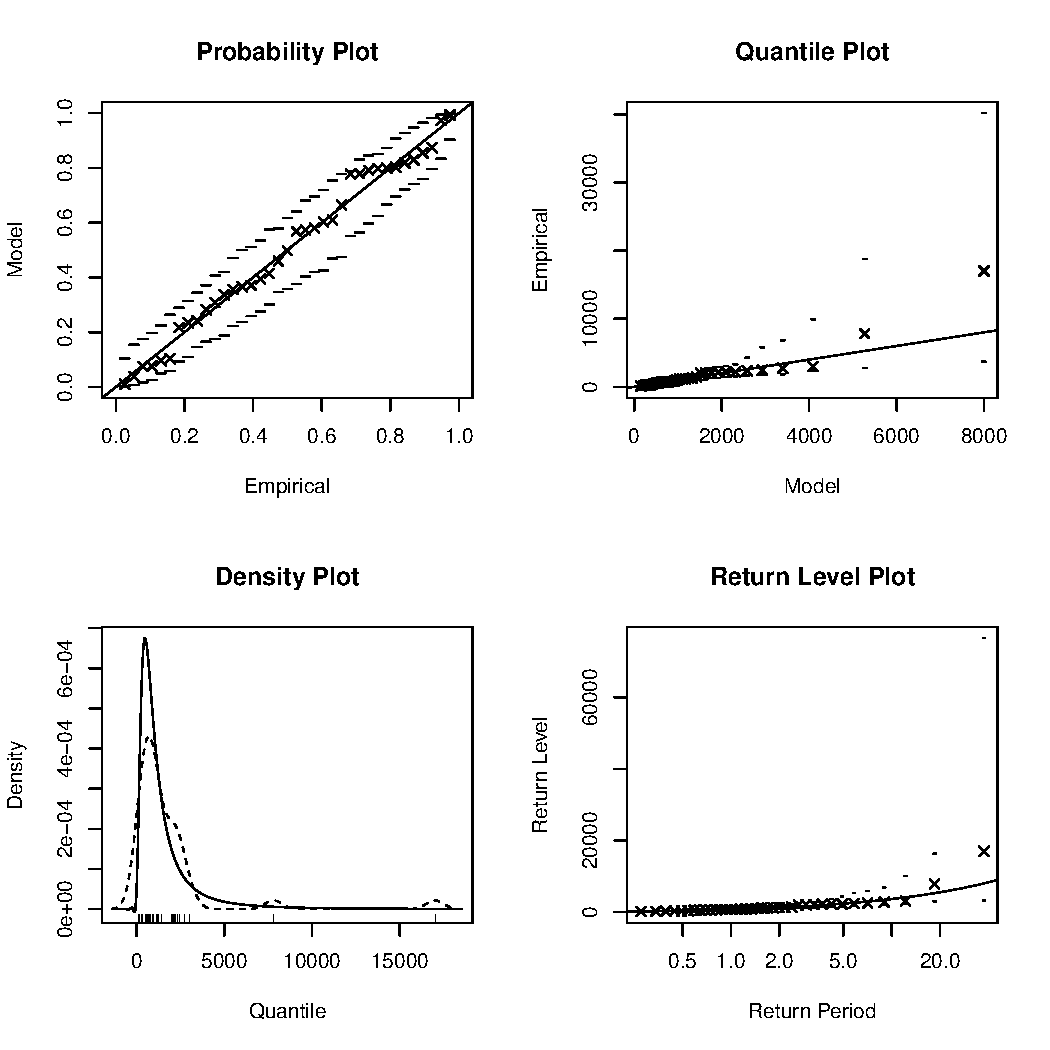
\includegraphics[width=0.35\textwidth]{../plots/monthly_mle_diag/01_monthly_mle_diag.pdf}\\
	\textbf{December}\\
	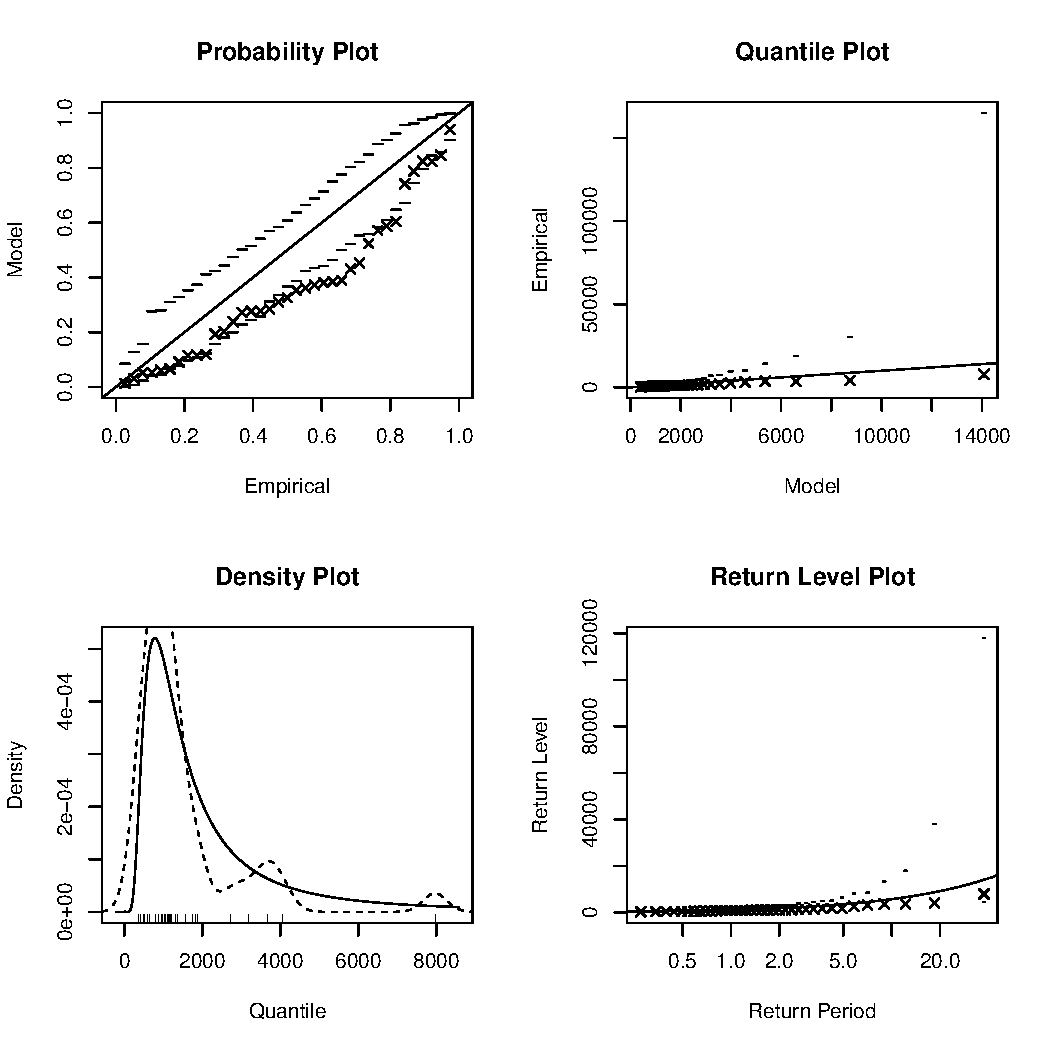
\includegraphics[width=0.35\textwidth]{../plots/monthly_mle_diag/12_monthly_mle_diag.pdf}
	\caption{Diagnostic plots for fitting GEV to the data using maximum likelihood estimation for January (top) and December (bottom). Whereas in January the model fits the data, as shown by the fact that the observed values are within the confidence range for probability plot, this is not the case for December, indicating a poor fit.}
	\label{fig:mle_diag}
\end{figure}
\par
First, we fitted the values using maximum likelihood estimation. Fitting was done using the evd package in R, using the Nelder-Mead optimization method and standard parameters \cite{evd}. The quality of the fit was assessed using diagnostic plots, as shown for January and December in Figure \ref{fig:mle_diag}. The model performed well with the exception of September and December: In September optimization didn't succeed, whereas in December the observed values lie outside of the given confidence intervals, as shown in Figure \ref{fig:mle_diag}. For both of these months, no standard error could be calculated due to singularity of the observed Fisher information matrix. Since we expect some continuity over the course of the year, the problem wasn't further investigated as inferences for the missing months can be made from their adjacent months. 
\par

\par
Then, we fitted the values using the Metropolis-Hastings algorithm. As a prior for the three parameters, a normal distribution with mean zero and a diagonal covariance matrix $\Sigma$ was used. 
WIE GENAU FUNKTIONIERT DS? I TSCHEGGES LEIDR NID SO GANZ...
The proposal standard deviations were fine-tuned to obtain acceptance rates between 0.2 and 0.4. In order to avoid having to fine-tune every month separately, we implemented the following very simple optimization algorithm: If the acceptance rates for a given parameter were too high, the proposal standard deviation for said parameter were multiplied with 1.5. In the opposite case for low acceptance rates, the proposal standard deviation was divided by 2. The Metropolis-Hastings algorithm was run with 30'000 iterations. The chain was thinned with a factor 300 in order to avoid dependence between steps of the markov chain. The thinning was validated with autocorrelation plots (not shown). The final parameter was determined to be the median of the posterior distribution, in order to be robust to outliers and be more adapted to skewed distributions. 
\par


\section*{Dependence of PROD on Time and ENSO}


\section*{Dependence of CAPE and SRH}
Asymptotic dependance (or independance) of bivariate maxima can be estimated using $\chi$ and $\bar{\chi}$ plots. The chi plot can be used to estimate dependance. The value of interest is $\chi = \lim_{u \to 1} \chi(u)$. For independance, $\chi \to 0$, since as $u \to 1$, $P\{F_X(x)>u | F_Y(y)>u\} \to \chi$. $\chi$ can distinguish the strength of dependence, but not the rate at which $\chi(u) \to 0$ as $u \to 1$. For this we can use the $\bar{\chi}$ plot. Generally we can say that for asymptotic independance $\lim_{u \to 1} \bar{\chi}(u) \to 0$, and for asymptotic dependance $\lim_{u \to 1} \bar{\chi}(u) \to 1$. (Source Slides 239-242 of the lecture notes)
\par
Our chi plots for all months look very similar. They suggest asymptotic independance between $CAPE$ and $SRH$ since $\lim_{u \to 1} \chi(u) \to 0$ and $\lim_{u \to 1} \bar{\chi}(u) \to 0$. Figure \ref{fig:cape_srh_chi} shows to represantative examples of the chi plots, for May and November. 

\begin{figure}
	\centering
	\textbf{May}\\
	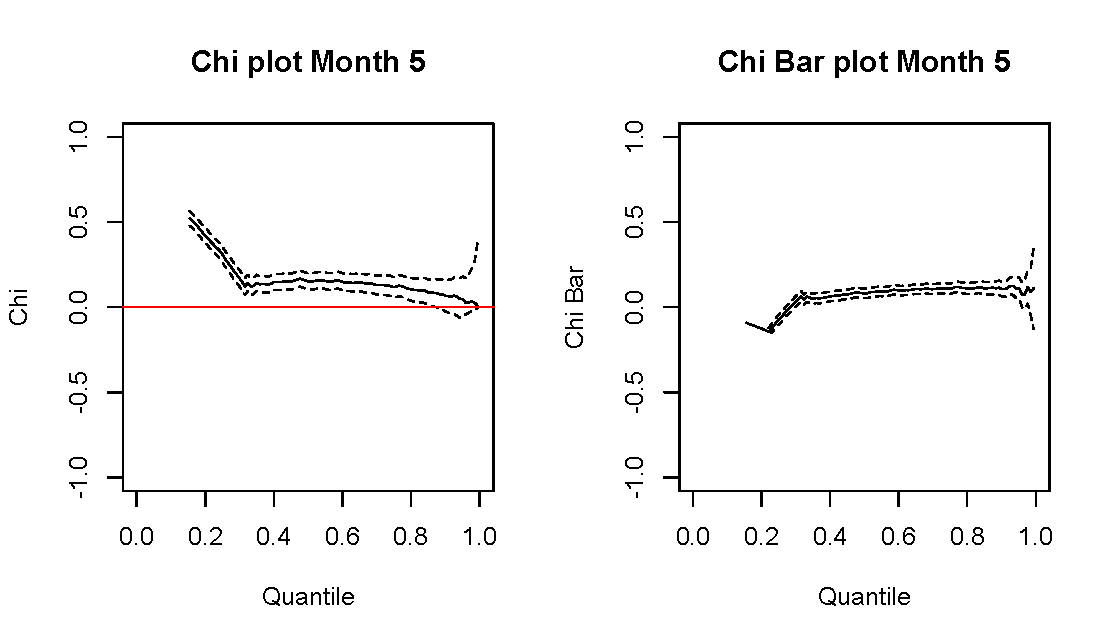
\includegraphics[width=0.35\textwidth]{../plots/May_chi.pdf}\\
	\textbf{November}\\
	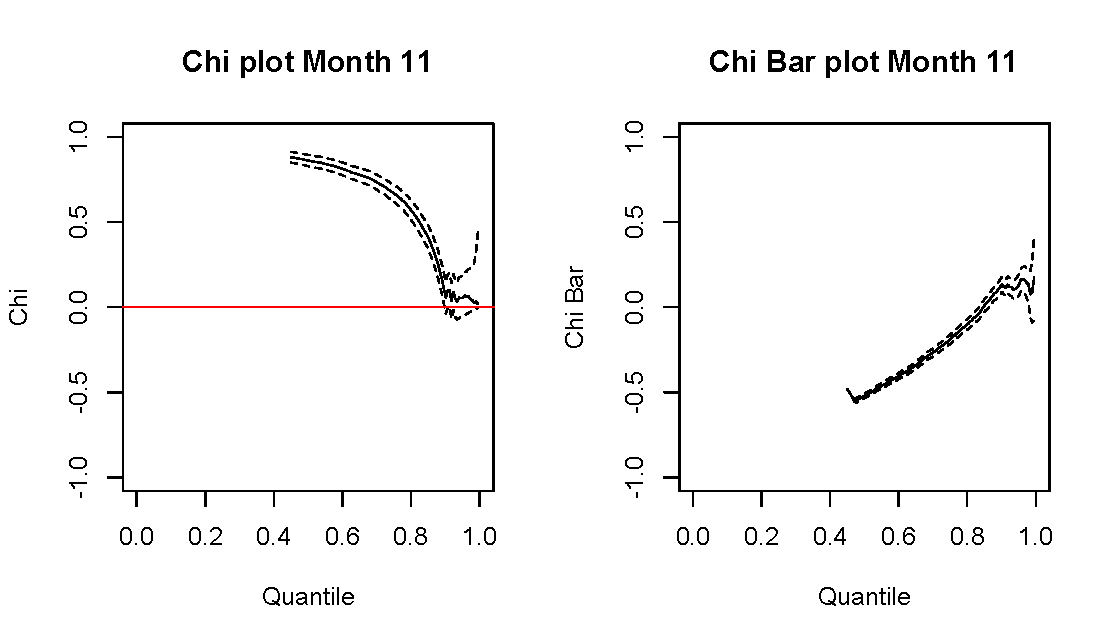
\includegraphics[width=0.35\textwidth]{../plots/November_chi.pdf}
	\caption{Representative examples for chi plots for $CAPE$ and $SRH$. Both suggesting asymptotic independance.}
	\label{fig:cape_srh_chi}
\end{figure}

\section*{Bivariate Fitting of CAPE and SRH}
When fitting the bivariate extreme value distribution, other than the parameters for the marginals, also the link function has to be estimated. We use a parametric link function, the different models araising from different link functions are compared using Akaike Information Criterion (AIC). We argue that there is no logical reson to use a different link function for different months, so we select the negative logistic model for estimating the return level later, it is always one of the best and if it has only small deviance from the best model if it isn't the best one. The models we compared are logistic (log), assymetric logistic (alog), negative logistic (neglog), bilogistic (bilog), Coles-Tawn (ct) and negative bilogistic (negbilog). The AIC comparison can be see in Table \ref{table:cape_srh_AIC}.
\begin{table}[]
\begin{tabular}{lllllll}
Month     & log       & alog      & neglog    & bilog     & ct        & negbilog  \\
January   & 920.4382  & 921.3970  & 920.1642  & 920.3145  & 921.0079  & 920.2859  \\
February  & 993.3549  & 997.1011  & 993.5037  & 995.2953  & 996.2297  & 994.7713  \\
March     & 1070.1139 & 1074.1772 & 1069.5276 & 1072.2210 & 1074.1263 & 1071.6125 \\
April     & 1064.8431 & 1068.7144 & 1064.6150 & 1066.1080 & 1066.2456 & 1066.3411 \\
May       & 1066.4916 & 1070.3846 & 1066.4539 & 1068.2524 & 1070.9600 & 1068.1580 \\
June      & 1043.2724 & 1047.0365 & 1043.4270 & 1040.6507 & 1043.1069 & 1045.4948 \\
July      & 1046.9983 & 1044.9287 & 1046.6727 & 1046.2317 & 1048.3972 & 1046.4537 \\
August    & 1029.1591 & 1032.9770 & 1029.4004 & 1031.1374 & 1031.2920 & 1031.1837 \\
September & 1056.0452 & 1059.5972 & 1055.6588 & 1058.0904 & 1059.8551 & 1057.3405 \\
October   & 1037.9838 & 1042.0191 & 1037.6208 & 1037.5553 & 1039.2542 & 1038.4781 \\
November  & 1012.4036 & 1016.4255 & 1012.3667 & 1014.5137 & 1015.1308 & 1014.0998 \\
December  & 892.7140  & 896.7475  & 892.5378  & 894.8876  & 895.4521  & 894.2789 
\end{tabular}
\caption{AIC comparison of different link function models}
\label{table:cape_srh_AIC}
\end{table}

For the fit, we extracted for each month the maximal $SRH$ value and the maximal $CAPE$ value and fitted the distribution to this data pair. We have therefore to be careful when drawing conclusions, since the "observations" we fit the models to often don't actually exist!

Before, we estimated the dependance between CAPE and SRH. We can also verify these results with the fits we just made. For this we will use the dependance parameter $\alpha$ from the logistic model. For this model, we know that for independance $\alpha \to 1$ and for complete dependance $\alpha \to 0$. In Figure \ref{fig:cape_srh_dependance_logistic} we plot the dependance parameters with 95\% confidence bands. This suggests that independance between $SRH$ and $CAPE$ cannot be ruled out, in accordance to our analysis in the previous paragraph.

\begin{figure}
	\centering
	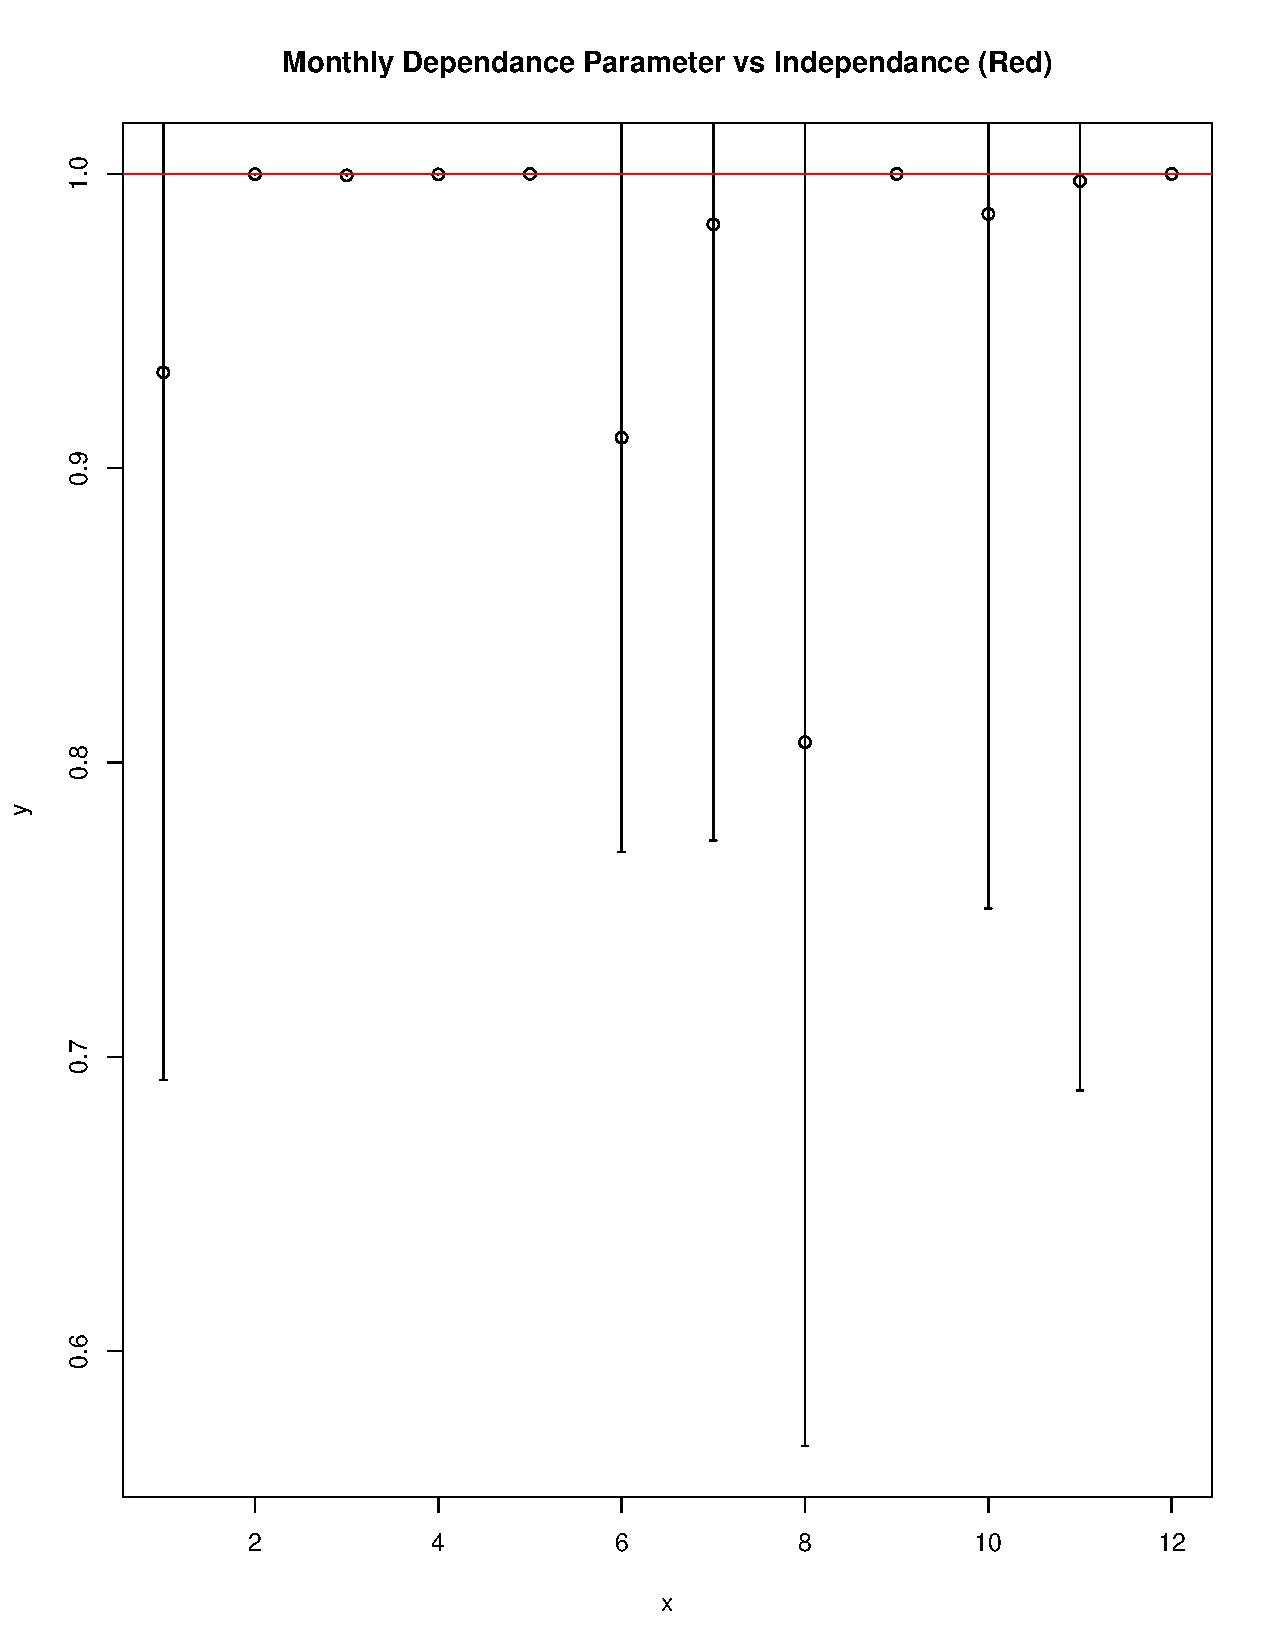
\includegraphics[width=0.35\textwidth]{../plots/dependance_parameter_cape_srh_logistic.pdf}
	\caption{Monthly dependance parameter $\alpha$ with 95\% confidence bands.}
	\label{fig:cape_srh_dependance_logistic}
\end{figure}

\section*{Calculation of Return Levels}

\section*{Impact by Using Variable Transfromations}

\section*{Conclusion}



%%% Bibliography
\bibliographystyle{IEEEtran}
\bibliography{literature-project}


	
\end{document}
